\documentclass{llncs}

\usepackage{graphicx}
\usepackage{ctable}
\usepackage{tabularx}
\usepackage{subfig}

\title{Workflows and Distributed Version Control}

\title{Workflows and Distributed Version Control}
\author{Olof Johansson \and Daniel Persson}
\institute{Blekinge Institute of Technology}

\begin{document}

\maketitle

\begin{abstract}
 This bachelor thesis focuses on distributed version control systems
 and workflows used when working with such systems. The thesis will
 investigate benefits and disadvantages in using distributed version
 control in software development using a literature review of the
 available articles on the subject as well as a post-mortem analysis
 (with questionnaires and data collected from the build environment) 
 of a student run software engineering project. We find that the
 migration costs are high, but that the advantages may outweigh its
 drawbacks for some. We conclude that many projects would benefit from
 migrating, but in particular, that new projects would not only
 benefit, but also not have high migration costs.
\end{abstract}

\section{Introduction}

We intend to investigate the adoption of the new trend within version
control systems (VCS) --- distributed version control systems (DVCS)
--- within the field of software engineering. The use of DVCS has
increased in the last years, with the introduction of several
implementations. The move from centralized version control to DVCS may
not always be unproblematic due to conceptual differences. It is
important to investigate the benefits and challenges of DVCS in order
to let software projects make informed decisions in their choice of,
and use of, version control systems. The research will be conducted as
a literature review, and as a post-mortem analysis of a student run
software project. The paper will try to answer the following questions:

\begin{enumerate}
 \item How do the developers adapt to a distributed workflow?
 \item How does a distributed workflow affect code quality in relation
       to the release management and code review?
\end{enumerate}

In Section \ref{sec:background} we introduce the concepts of VCS and
give a brief history of its evolution. In Section \ref{sec:telia} we
introduce the student run Telia Smart Home project with focus of its
use of version control systems. The primary means of doing the
post-mortem analysis will be to conduct interviews with participants
in their various roles. In addition to this we will also collect data
from various project management and configuration management tools and
systems.

\section{Background}
\label{sec:background}

The history of Version Control Systems can be divided into three
categories; the ones that only manages local files, the ones that rely
on a central server to serve connecting clients, and finally the
distributed ones, where every 'node' can act as both a client and a
server. The three categories roughly follow each other
chronologically, naturally with transition-periods in between. At the
moment the dominating tools are mostly client-server, but the
distributed ones are rising fast in popularity, so perhaps we are
currently in the start of a new transition.

\subsection{The Local Era}
The first VCS ever released was the \emph{Source Code Control System}
(SCCS) in 1972. SCCS tried to solve a number of problems that software
developers of that time had. Manually managing several versions of the
same product simultaneously was not feasible in the long run for
several reasons described by the creator of SCCS, Marc J. Rochkind
\cite{rochkind75}:

\begin{itemize}
 \item The amount of space to store the source code may be several
       times that needed for any particular version.
 \item Fixes made to one version sometimes fail to get made to
       other versions.
 \item When changes occur it is difficult to tell exactly what changed
       and when.
 \item When a customer has a problem it is hard to figure out what
       version he has.
\end{itemize}

Instead of saving entire files in various states, SCCS stores the
differences between versions of the same file (called diffs, or
deltas\cite{ambriola90}). With each delta SCCS also stores metadata
such as who made the change, why, and when. This did not only save
precious storage space, but also provided the \emph{traceability} that
the software developers had previously lacked\cite{rochkind75}.

It is worth noting that SCCS was not the only VCS that followed the
philosophy of storing the files locally, \emph{Revision Control
System} (RCS) which was essentially a wrapper around the Unix tool
\emph{diff} was released in 1982 and gradually started taking over as
the dominant VCS for Unix\cite{tichy85}.

\subsection{The Client-Server Era}
Although RCS was an improvement over SCCS it still had several flaws;
it was still operating on single files only, and they were still
stored locally. 

To be able to cooperate with his students, working on differing
schedules, Dick Grune created shell scripts to centrally manage the
project they were working on through RCS\cite{grune86}. When the
project was over he realized the potential and cleaned up the scripts
and published them in late 1985. Two years later Brian Berliner
rewrote the software in C, and CVS was born.

CVS introduced all the modern terminology we use today when we talk
about version control\cite{cederqvist93}; the code is stored in a
\emph{repository} that users can \emph{check out} a \emph{working
  copy} from. Terms such as \emph{committing} code and \emph{merging}
changes was also introduced by CVS. It also made \emph{branching} a
bit less cumbersome than it had been in RCS although merging the
branches still required a lot of work.

With CVS in the front line and with proprietary version control
systems starting to pop up in the early nineties the model of a
central server that contained the repository that everyone worked in
became the standard way to think about version control.

Although CVS simplified and popularized the use of version control
systems it has still received its fair share of
criticism\cite{robert06}\cite{subversion}: For example the revision
numbers are created on a per file basis, which means that the latest
revision number is not the same across the board which can sometimes
be confusing. Other things like not handling symbolic links for
example is claimed by the CVS developers to be carefully planned
features (in the case of symbolic links due to security concerns)
rather than bugs, but as the issues started to pile up Collabnet
(founded by Tim O'Reilly that founded \emph{O'Reilly Media} and Brian
Behlendorf, co-founder of the Apache project) started the Subversion
project.

Subversion was released in 2000, and solved many of the issues that
CVS had, while still maintaining the same working style of
CVS. Subversion didn't really introduce any revolutionary ideas, but
rather focused on the weaknesses of CVS like versioning of symbolic
links, versioning for directories and file metadata and truly atomic
commits (meaning if the transmission between client and server is
interrupted, the commit is rolled back rather than processed half-way,
much like transaction in a database\cite{subversion} --- in CVS this
wasn't the case, and it could cause inconsistencies or corrupted data
if it happened).

Other systems such as IBM's ClearCase and Microsoft's Visual
SourceSafe and Team Foundation Server existed, but never reached the
same popularity as CVS (that even to date manages a significant amount
of projects) and Subversion (that is currently the most popular tool
for version control) due to its proprietary licensing.

\subsection{The Distributed Era}

The next innovation came from the open source community, where the
centralized approach of CVS and Subversion didn't come as natural as
it perhaps does in the corporate domain. Instead of storing the
repository on a centralized server, distributed version control
systems like GNU Arch, Monotone and Mercurial (hg\footnote{
 The "abbreviation" comes from the symbol for mercury in the periodic
 table.
}) stored a copy of the repository on every client that checked out a
working copy. That way developers could always have access to the full
history even without an internet connection. 

One of the first distributed version control systems, BitKeeper,
infamously withdrew the rights for the Linux kernel project to freely
use BitKeeper\cite{robert06}\cite{shaikh02} (which was a proprietary
system) which sparked Linus Torvalds to create a new, free tool: Git.

The main goal with git was to create a version control system that
supported a BitKeeper-like workflow with high performance and strong
integrity control. Since Linus also has a passionate hatred for CVS he
has also said ironically that if there is any doubt in any design
choice to be made, the opposite of the one CVS took is the way to
go\cite{torvalds07}.

Git has in the past few years seen a steady growth in users and
projects, and while the numbers compared to Subversion is still quite
small, the change speed is pointing straight up\cite{bird09}.

\section{Research Methodology}

To answer the research questions proposed in the introduction we will
conduct both a review of literature in the field of configuration
management in general, and version control systems in particular, and
then conduct a post-mortem analysis of the Telia Smart Home
project. The primary means of doing the post-mortem analysis will be
to conduct interviews with participants of the student projects in their
various roles. In addition to this we will also collect data from
various project management and configuration management tools and
systems (eg. Jenkins, Git or Redmine).

\subsection{Literature Review Design}

To provide a foundation for our thesis we will look at papers relating
to centralized and decentralized version control, to give a clear view
of what the differences between the two are, from a user perspective
--- i.e. in terms of migration costs, conceptual difference et cetera.
Especially interesting is what kind of workflows that the DVCS tools
enable, and compare it to the workflow used by the Telia Smart Home
project.

After a preliminary survey of the available material on the topic we
have noticed that scientific material regarding this is quite scarce,
and we therefore choose not to provide any exact search strings, but
instead decide to limit ourself to the domains of configuration
management in general, and version control systems in particular, and
also provide a list of keywords that search-strings can be composed
of: 

\begin{itemize}
 \item VCS, Version Control
 \item DVCS, Distributed Version Control
 \item SCM, Source Control Management
 \item Git, Subversion, Mercurial, Perforce, Darcs, CVS, BitKeeper
 \item Checkin, Checkout, Commit, Diff, Branch, Merge, Rebase
 \item Configuration Management
\end{itemize}

We will focus our searches at Google Scholar and Elin, but if needed
we will also resort to using for example IEEE Xplore or other relevant
tools. In worst case, we will also use of white papers or other
sources not published in academic papers (e.g. performance tests
conducted by hackers and other non-academics).

The initial screening will be done by reading abstracts and
conclusions to quickly dismiss irrelevant papers, and the go through
the most promising candidates more thoroughly to decide what to use.

\subsection{Post-mortem Analysis Design}

The post-mortem analysis will primarily be based on interviews with
participants in the Telia Smart Home project and questionnaries with
members from other projects within the same course framework. We will
base the interviews and questionnaries around these questions:

For the participants in the Telia Smart Home project we asked the
following questions:

\begin{enumerate}
 \item How would you rate your proficiency in using Distributed
       Version Control Systems? (scale 1-5)
 \item How would you rate your proficiency in using Version Control
       Systems? (scale 1-5)
 \item Do you have any previous experience with VCS? If so, please
       describe.
 \item What benefits do you see in using the workflow employed by the
       Telia Smart Home project?
 \item What drawbacks do you see in using the workflow employed by the
       Telia Smart Home project?
 \item Do you have any suggestions for improvements?
 \item What is your overall opinion of the workflow?
 \item Would you advice others to use the workflow? (yes/no)
\end{enumerate}

For the participants in the other projects (within the same course
framework) we sent out a subset of the survey as they did not employ
the same workflow as the Telia Smart Home project:

\begin{enumerate}
 \item How would you rate your proficiency in using Distributed
       Version Control Systems? (scale 1-5)
 \item How would you rate your proficiency in using Version Control
       Systems? (scale 1-5)
 \item What VCS software have you used before?
 \item Do you have any previous experience with VCS? If so, please
       describe.
 \item What Version control software are you currently using?
 \item How do you work with your VCS tools?
 \item Would you advice others to use your workflow? (yes/no)
\end{enumerate}

The post-mortem analysis will also include an analysis of various data
collected during the project. Most of this data will come from
different configuration and project management tools, such as Git for
Version Control, Jenkins for continuous integration or Redmine for
time management and issue tracking.

The data collected from the project and configuration management tools
will then be correlated with the data gained from the interviews and
questionnaries.

\section{Literature Review}

%* in common
\subsection{Adoption}

In these next few sections we will try to answer research question 1.

\subsubsection{Migration Costs}

There a large number of open source as well as proprietary projects
moving to one of the major distributed version control system; Perl,
Curl and Parrot are projects that all has migrated to Git, from their
earlier centralized VCSes\footnote{
 Perl migrated from Perforce, Curl from CVS and Parrot from Subversion.
}. The migrations has not always been cheap, e.g. the Perl migration 
took 22 months \cite{alwis09}, so they must have had good reasons to 
do it. We will try to see why this might have been in the next few
subsections.

A migration of VCS is twofold. There is migration of the repository,
with moving every commit with its meta data and authorship
information, every branch and every tag to the new VCS, making sure
that nothing is lost and that nothing is broken. A problem in its own
right, but with a lot of tools available producing generally good
results. The other side, however, is migrating the developers and the
workflows. Changes in interface design requires every developer to
"relearn" the various actions and tools used. Something as trivial as
commit IDs are different and has become a problem for some
\cite{alwis09} --- the centralized VCSes commonly use incremental
integers to identify a commit; DVCSes usually use a checksum of the
content instead. The incrementing integers says more to a human when
comparing two commits, which of the two commits are the newest, and
perhaps gives a hint about how much newer \cite{bird09}. The loss is
an unfortunate effect of the distributed nature of DVCS. As every
repository is "isolated" from each other, and only interacts when
merging with each other, they can not know what numeric ID they should
give to a commit to make it globally unique and still retain the
incremental property.  So instead checksums are used; well known
algorithms are used to calculate a large value based on the contents
of the commit. This difference between DVCS and VCS is one of the
first a new DVCS user encounters.

Another change from centralized VCS is the decoupling of committing
and merging. This makes it a two command operation to do the
equivalent of "svn commit". Looking past the short term
impracticalities of having to do two commands to merge with a central
server, it gives the developer freedom to not merge at all, or not
merge "right now". Perhaps it is not even possible to merge --- as is
the case in airplanes or being in remote areas and no network
connectivity is available.

An other change, not a change in the interface but a change of VCS
nomenclature, is perhaps an even bigger obstacle for migration
\cite{bird09}. Some words are introduced, some words are removed and
some words are redefined. Committing is, as described, no longer
publishing your changes in the central repository. Pulling and pushing
are common words within DVCS for things that don't even exist in a
centralized VCS. In short, there will have to be a lot of
documentation of procedures, tools and workflows when migrating to a
new VCS --- especially a DVCS \cite{alwis09}.

\subsubsection{Architecture}

As mentioned in the section on migration costs, the fundamental
differences in the distributed version control architecture vis a vis 
the centralized ditto makes it hard to transfer workflows and
techniques directly. The differences do make it possible to other
things and brings number of benefits together with its disadvantages.

The distributed nature means that you have certain limitations on what
can be done to enforce synchronization: e.g. there is no file locking
support (making sure that only one developer works on a certain file
at a time) \cite{osullivan09} and it's harder to impose automated
content control. It makes it hard to delete history --- this would
have been problematic for e.g. the FreeBSD developers when they were
forced by a court decision to cease distribution of certain older
components \cite{alwis09}. But by the same token, it works as an
implicit distributed backup system, where each checked out repository
is a repository in its own right. Data loss at a single node won't be
a critical issue, as the complete repository with content and history
is replicated numerous times \cite{alwis09}. Another benefit from the
distributed architecture of DVCS is the ability to work independently,
isolated from the central repository. With this, a developer could
work when travelling to or from remote offices or conferences
\cite{alwis09}\cite{robert06}.

The research done in the field has largely depended on the activities
of various open source projects, with its wealth of openly accessible
data and discussions \cite{alwis09}\cite{bird09}. These kind of
projects has some specific problems and needs, some which only has a
limited effect on non open source projects. One positive effect of
distributed version control systems is that it lowers the bar for new
contributors. They can easily fork a project and commit changes, and
then make a request to be merged into the mainline \cite{alwis09}.
This limits the phenomenon known as "commit whoring" or "commit
politics", where people try to get commit access just for the sake of
it (as a status symbol).

\subsubsection{Performance}

The fact that anyone using a DVCS is working with a local repository
has big impacts on performance. In a CVCS every operation requires
access to the central server, and thus adds network latency to every
operation\cite{torvalds07}. Additionally, every developer that works
towards the same central server adds more to its workload, making it
scale quite badly. In contrast, DVCSes do not work towards the same
server, even though some repositories are perhaps considered 'more
important' than others, and thus scales very well almost any amount of
developers\cite{shaikh02}. Working locally leads to operations like
branching and merging being much faster and smoother, encouraging
developers to use them more\cite{alwis09}.

\subsection{Quality Implications}
In this section we will try to answer research question 1.

The fact that most operations are so fast in DVCSes will have an
impact on how people work with their SCM tools. The fact that
branching is such a cheap operation will encourage developers to
actually use branches where they see fit, without taking things like
workload on a central server, namespace pollution, or wait times into
consideration. Coupled with the fact that merging branches is
relatively painless --- and thus resulting in merging being done when it
should, instead of being postponed to delay the suffering for the
developer, creating unnecessary conflicts and more suffering --- will
in turn lead to a more thorough and in a sense more correct use of the
VCS, resulting in a better history and potentially better code.

Another powerful tool that can be used more frequently due to the huge
performance-benefits that DVCSes provide is \verb!bisect!. It is very
easy to use, but can prove to be very useful in finding bugs, or
rather finding out when they are introduced. What \verb!bisect! does
is basically a binary search between two revisions (between which you
know that a bug is introduced) by checking out revisions and asking
the developer if the bug is present or not. Provided that the bug can
be replicated with for example a script, this task can be automated
fairly easy, and the fact that everything runs locally keeps the
performance up, and prevents the network from being congested.
Needless to say, when looking for a particular bug it is a huge
advantage to know the exact commit that introduced it.

Since the primary mean of sharing and spreading code in a DVCS
workflow is by pulling other peoples changes into a local repository,
introducing quality practices like \emph{code reviews} fits in very
well. Whenever anyone pull code from someone else, they simply look at
the diff, and if it does not meet the agreed upon quality standards,
they don't merge them until they do\cite{osullivan09}.

\section{The Telia Smart Home Project Context}
\label{sec:telia}

The last semester of the Software Engineering program at Blekinge
Institute of Technology is concluded with a large group software
engineering project. Within this course, the students are put in
charge of themselves organizing and execution a software project for a
customer from the industry. The authors of this paper participated in
one such project, \emph{Telia Smart Home}. The project team consisted
of eight students. The choice of project methodology and tools was put
in the hands of the students.

When choosing a VCS the project members had a number of considerations
to account for. VCS can be used in a number of ways. Some limits are
posed by the choice of tools. Subversion is built for centralized
version control, whereas tools like git or mercurial are built for
decentralized. Members of the latter category are generally more
flexible; e.g. git is almost as simple to run centralized as running
it decentralized as it is intended. The Telia Smart Home project has
chosen to use git. The reasons for this are several: the ability to
use git decentralized as well a centralized was a major point. Also,
the prior experience from some members of the project made the
transition for other members less burdensome.

But defining a workflow does not end with selecting a tool. As stated, 
git is very flexible in the way developers interact with it. It is not
uncommon to use it centralized, and in fact, the Telia Smart Home project
does just this in their documentation repository. But one of the key 
strength is its decentralization. It has no enforced "central repository"
through which all changesets must pass. If the team want to have a 
centralized repository it must itself give a arbitrary repository that
semantic meaning.

Are there any alternatives to be considered? Certainly. Again, git is 
indeed quite flexible. It will yield to the wishes of the user. There are 
a number of easily recognized workflows (perhaps not always mutually
exclusive). Some of the most popular ones are presented here:

\begin{itemize}
 \item \textbf{Centralized}: 
  Using git in a way similar to e.g. Subversion or other more traditional
  tools still give the user some advantages. The process of branching and
  merging is many times more well developed in git than it is in tools like
  Subversion. A property of the distributed nature of git gives yet another
  benefit: having all of the history available locally. You don't need
  network to be able to see what changes was introduced to a particular
  commit, and indeed no network to be able to see the commit log.

 \item \textbf{Topic branches}: 
  Working on a new cool, but experimental feature? Perhaps it is not as 
  tested as the rest of the system is. You probably don't want to have 
  it in the main code. Create a branch specifically for this "topic" or
  "feature".

 \item \textbf{Benevolent dictator}: 
  A workflow, especially popular within open source projects, is the
  benevolent dictator workflow. There is one designated maintainer, and
  other contributers make "pull requests", primarily via e-mail.  If the
  benevolent dictator accepts the patch, he or she merges it into his or
  hers own repository, where everybody gets their source code from. The
  name, "Benevolent dictator", is a term jokingly used about Linus
  Torvalds, the initial author and later primary maintainer for the Linux
  kernel (and also, the initial author of git!).
\end{itemize}

\begin{figure}[tp]
 \begin{center}
  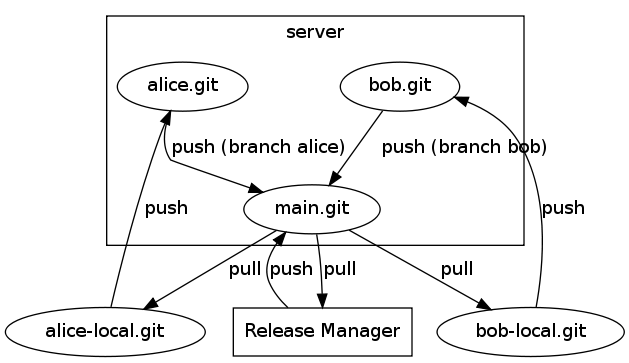
\includegraphics[scale=0.5]{workflow.png}
  \caption{Workflow description}
  \label{fig:workflow}
 \end{center}
\end{figure}

Each of these workflows are appropriate in some situations. However,
none of these totally fitted the needs of the Telia project. Instead,
the Telia Smart Home project designed its own workflow (see Figure
\ref{fig:workflow}). The workflow used for the code repositories in the
project is based upon individual developer repositories and branches.
Each developer has an own repository, and makes commits to this. The
system (with the help of so called hooks (i.e. scripts triggered by
specific events)) then pushes changes to a repository on a central build
server. Here, a build is triggered using the \emph{Jenkins} continuous
integration system and the commit is also forwarded to the so called
"baseline" repository, but only to a developer's private branch. It is
not merged into the actual baseline code, but it is still accessible for
other developers.

The release manager is now notified that there is a commit awaiting
approval. He or she can check build and test status on Jenkins and see the
delta between baseline and the proposed patch. After possibly running local
tests, the release manager can either approve and merge the commit or
reject it, and inform the author of why it wasn't suitable for inclusion.
If the commit is merged, other developers are now encouraged to merge it 
into their local repositories, their working copy of the source code. 

When designing this system, the sought benefits was the integrated code 
review and approval system. With this, the release managers could validate 
adherence to coding conventions as well as making sure that the system
is buildable and all unit tests passes. Possibly, much of this could even
have been automated (e.g. static code analysis and coding style validation
tools are commonplace) to an even higher degree, but that is, as always, a 
cost/benefit question. It is innovative and unique, but it does build upon
the so called "benevolent dictator" workflow, especially the release
management component of it. The success of this workflow from high-profile 
projects like the Linux kernel has been an inspiration for the design.
The reason why the project rejected the topic branch workflow at an early
stage was the problems associated with topic branches in the early stages
of a software project, where a lot of interdependencies exist and basic
infrastructure is needed. In later stages of the project, this workflow
would have been more feasible, but the overhead associated with switching
workflow was deemed to high. It has been used in some rare cases, where code
was at a very experimental stage.

\section{Results from Post-mortem Analysis}

From the conducted interviews it is noticeable that survey participants
rated their proficiency with DVCSes the same as with VCSes in general.

Regarding the workflow employed by the Telia Smart Home (TSH)
project, the survey conducted resulted in generally positive feedback,
with only some minor reservations. Some concern was raised regarding
the way the project ``abused git'' in the way branches were
automatically re-pushed to branches in the mainline
repository. A problem with the release manager approach was that it
easily becomes a bottleneck, if for example the release manager is
absent or busy. Several survey participants claimed to have
experienced this problem. Another survey participant noted that the
workflow looked more complex than it really was. Other participants
noted that the code review came natural and worked well, and that the
mainline build was rarely broken.

\begin{table}[tp]
 \begin{center}
  \begin{tabular}{ccc}
   \toprule
   Date & Build attempts & Duration (min) \\
   \midrule
   2011-03-10 & 2 & 5 \\
   2011-03-10 & 3 & 21 \\
   2011-03-11 & 1 & 49 \\
   2011-03-11 & 1 & 4 \\
   2011-03-14 & 1 & 25 \\
   2011-03-30 & 11 & 115 \\
   \bottomrule
   \\[-0.7em]
  \end{tabular}
  \caption{Statistics for build failures}
  \label{tbl:breakage}
 \end{center}
\end{table}

\begin{figure}[tp]
 \begin{center}
  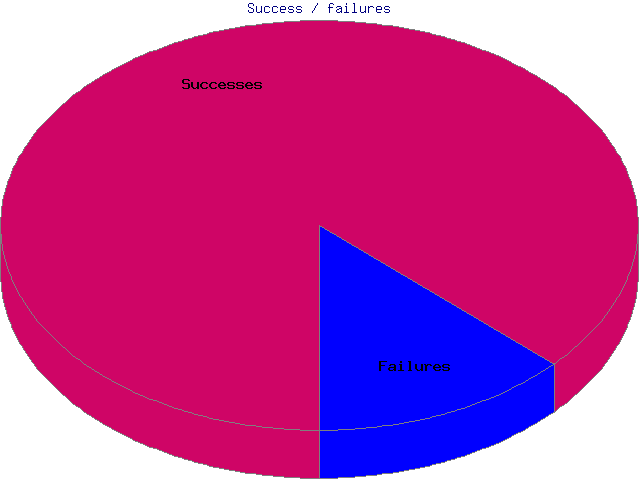
\includegraphics[width=0.8\textwidth]{binary-blobs/pie}
  \caption{The percentage of successful builds (red) and failed
           builds (blue) within the Telia Smart Home project, over a
           period of 153 builds.}
  \label{fig:successbuilds}
 \end{center}
\end{figure}

Comparing to the data collected from the continuous integration
environment (Jenkins) we can easily see some indications of the
project quality state:

\begin{itemize}
 \item The number of successful builds represents 86.85\% of all
       builds. See Figure \ref{fig:successbuilds}. 
 \item The average time it took to fix a build failure\footnote{
        A build failure is defined as either a compilation error, 
        one or more failing unit tests or problems in the build 
        environment.
       } was 30 minutes, with a mean time of 21 minutes. See Table
       \ref{tbl:breakage}.
 \item There were no build errors after 2011-03-30. See Table
       \ref{tbl:breakage}.
\end{itemize}

It is hard to know what kind of impact the release management approach
used by the project had without control data, but the situation was
satisfactory for the project. The fact that build was only broken in
the beginning of the project could be an indication that the release
management was effective once the team and release managers got used
to the workflow.

When looking at the survey results from the participants in other
projects, the general impression is that little though has been put
into the design of their VCS workflows. Only a minority of the
respondents "understood" what \emph{workflow} meant, in the VCS
context. Those that did, described a simple centralized workflow ---
with or without DVCS tools. 

\begin{figure}
 \begin{center}
  \subfloat[Previous experience with VCS tools]{
  \label{fig:vcsused}
  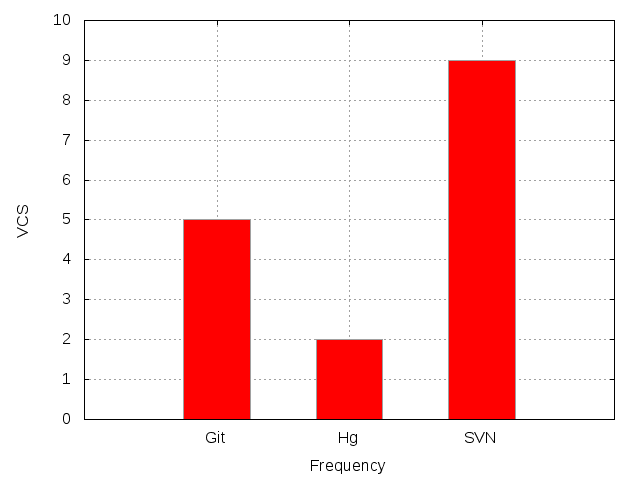
\includegraphics[width=0.8\textwidth]{binary-blobs/vcs-used}
 }
 \\
 \subfloat[Proficiency with VCS and DVCS]{
  \label{fig:vcsprof}
   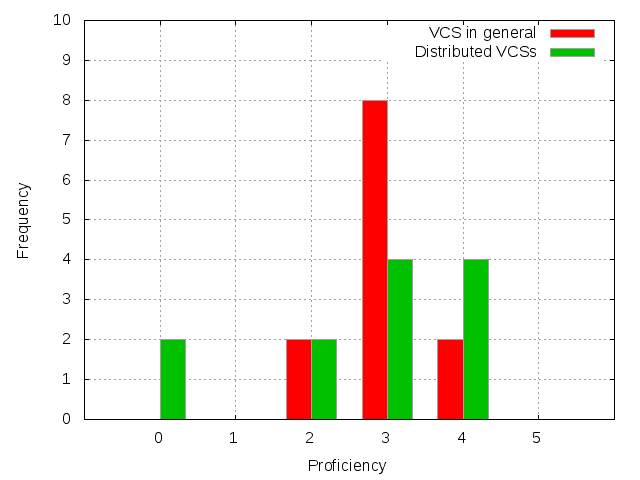
\includegraphics[width=0.8\textwidth]{binary-blobs/vcs-prof}
 }
 \caption{Results from survey with external project participants}
 \end{center}
\end{figure}

Another observation was that almost half of the respondents had never
used a version control system until the current project. Those that
did have prior experience had used primarily Git or Subversion, with
some minor use of Mercurial also accounted for. The respondents
stated that they had prior experience with Mercurial did not report
that they had used Git. See Figure \ref{fig:vcsused}. Most of the
respondents described their current proficiency level with VCS in
general as a "three" on a scale from one to five. The DVCS proficiency
was centered around three and four on the same scale. See Figure
\ref{fig:vcsprof}.

\subsection{Analysis of Post-Mortem Findings}
The survey responses within the Telia Smart Home project made it clear
to use that the workflow was feasible and that the developers
unanimously was happy with it, albeit with some minor criticism.

The re-pushing of branches could very well have been excluded from the
workflow, the reasons for having it was to ease the work for release
managers by having all changes in one repository and not spread
out. The other reason was to allow easy overview in the issue tracking
system (Redmine) which was limited to only show one repository.

The release management criticism is not in any way limited to the TSH
workflow, it is present in any workflow using a review process to
accept and merge commits. One possible solution could be for example
having a dedicated person for the review process, but in this project
the cost would have been too big. Sharing the responsibility of
release management between several people could also remove the
downtime of the review process when the release manager is
absent. Overall the release management and code review has worked
well, with few hick-ups, and as Table \ref{tbl:breakage} shows, the
mainline build was broken relatively few times, and only for short
periods of time.

\section{Discussion}

The literature review focused on migration cost, whereas the
post-mortem analysis investigated the adoption of DVCS in a new
project. The migration in the latter case was an individual adoption
rather than the "collective" project migration usually described in
the literature. Still, some of the conclusions clash with the findings
in the literature review. The papers dealing with migrations
emphasize the problems with individual developers having to adopt to
new interfaces and changed behavior. During the course of the project,
this has been in large a non-issue. We suspect that we would find
other results if we would enlarge the scope of the research and
include a more diverse target group with more experience of software
engineering and version control.

\section{Conclusion}

\bibliographystyle{plain} 
\bibliography{references}

\newpage
\section*{Appendices}
\appendix
\section{Data from Literature Review}
\subsection{Version Management Tools: CVS to BK in the Linux Kernel}

An article by M. Shaikh and T. Cornford, written in 2002 and published 
in 3rd Workshop on Open Source Software Engineering.

\begin{abstract}
 Version management tools might be seen as a prerequisite for open
 source development today as projects become too large to be managed by
 maintainers alone. Yet the OS\footnote{ 
  OS, as in Open Source. Not to be confused with Operating System, our 
  comment.
 } process depends on fluid coordination and collaboration with the
 underlying qualities of this process based on firm trust and
 respect for fellow developers. This paper is a study of how
 debate over version tools reflects governance and decision making
 in an OS community. The paper is based on a study of the Linux kernel
 community as it first saw a partial acceptance of the CVS tool, and then
 later adopted BK\footnote{
  Bitkeeper, a proprietary version control system, our comment. 
 }. The paper explains the adoption process in relation to governance
 concerns, license issues, and questions of technical performance.
\end{abstract}

The described problems with introducing a distributed version control
system into a such a large project as the Linux kernel, may give us
insight into the adaption process. This paper relates to research
question 1.

\subsection{Making Sense of Revision-Control Systems}

An article by B. O'Sullivan, written in 2009 and published in
Communications of the ACM.

\begin{abstract}
 All revision-control systems come with complicated sets of trade-offs. How
 do you find the best match between tool and team?
\end{abstract}

A high-level description of revision control tools and concepts and its use
will give us a reference on what properties is interesting in version
control workflows.

\subsection{Darcs: Distributed Version Management in Haskell}

An article by D. Roundy, written in 2005 and published in Proceedings of the
2005 ACM SIGPLAN workshop on Haskell.

\begin{abstract}
 A common reaction from people who hear about darcs, the source control
 system I created, is that I sounds like a great tool, but it is a shame
 that it is written in Haskell. People think that because darcs is written
 in Haskell it will be a slow memory hog with very few contributors to the
 project. I will give a somewhat historical overview of my experiences with
 the Haskell language, libraries and tools.

 I will begin with a brief overview of the darcs advanced revision control
 system, how it works and how it differs form other version control systems.
 Then I will go through various problems and successes I have had in using
 the Haskell language and libraries in darcs, roughly in the order I
 encountered them. In the process I will give a bit of a tour through the
 darcs source code. In each case, I will tell about the problem I wanted to
 solve, what I tried, how it worked, and how it might have worked better (if
 that is possible).
\end{abstract}

A case study into a specific distributed version control system. Even
though the paper deals in large parts with the implementation details,
the actual usage and interaction with the system is described. This
paper relates to research question 1.

\subsection{Towards a Better SCM: Revlog and Mercurial}

An article by M. Mackall, written in 2006 and published in the Linux
Symposium.

\begin{abstract}
 Large projects need scalable, performant, and robust software configuration
 management systems. If common revision control operations are not cheap,
 they present a large barrier to proper software engineering practice. This
 paper will investigate the theoretical limits on SCM performance, and
 examines how existing systems fall short of those ideals.

 I then describe the Revlog data storage scheme created for the Mercurial
 SCM. The Revlog scheme allows all common SCM operations to be performed in
 near-optimal time, while providing excellent compression and robustness. 

 Finally, I look at how a full distributed SCM (Mercurial) is built on top
 of the Revlog scheme, some of the pitfalls we've surmounted in on-disk
 layout and I/O performance and the protocols used to efficiently
 communicate between repositories.
\end{abstract}

Yet another case study into a specific distributed version control
system.  Again, this also deals with technical details, but the
interaction and usage pattern is interesting for our research. This
paper relates to research question 1.

\subsection{The Promises and Perils of Mining Git}

An article by C Bird, P. C. Rigby, E. T. Barr, D. J. Hamilton, D. M. German
and P Devanbu, written in 2009 and published in 2009 6th IEEE International 
Working Conference on Mining Software Repositories.

\begin{abstract}
 We are now witnessing the rapid growth of decentralized source code
 management (DSCM) systems, in which every developer has her own repository.
 DCSMs facilitate a style of collaboration in which work output can flow
 sideways (and privately) between collaborators, rather than always up and
 down (and publicly) via a central repository. Decentralization comes with
 both the promise of new data and the peril of its misinterpretation. We
 focus on git, a very popular DSCM used in high-profile projects.
 Decentralization, and other features of git, such as automatically recorded
 contributor attribution, lead to richer content histories, giving rise to
 new questions such as "How do contributions flow between developers to the
 official project repository?" However, there are pitfalls. Commits may be
 reordered, deleted, or edited as they move between repositories. The
 semantics of terms common to SCMs and DSCMs sometimes differ markedly,
 potentially creating confusion. For example, a commit is immediately
 visible to all developers in centralized SCMs, but not in DSCMs. Our goal
 is to help researchers interested in DSCMs avoid these and other perils
 when mining and analyzing git data.
\end{abstract}

And a third (and final) case study into a specific version control
system.  This paper does not primarily deal with technical details
however, and instead focusing on interaction details. This paper
relates to research question 1.

\subsection{Why Are Software Projects Moving From Centralized to
               Decentralized Version Control Systems?}

An article by D. de Alwis and J. Sillito, written in 2009 and published in 
2009 ICSE Workshop on Cooperative and Human Aspects on Software
Engineering.

\begin{abstract}
 Version control systems are essential for co-ordinating work on a software
 project. A number of open- and closed-source projects are proposing to
 move, or have already moved, their source code repositories from a
 centralized version control system (CVCS) to a decentralized version
 control system (DVCS). In this paper we summarize the differences between a
 CVCS and a DVCS, and describe some of the rationales and perceived benefits
 offered by projects to justify the transition.
\end{abstract}

This paper is relevant to us and important for us to understand the reasons
for migration, and as a reference for comparisons with centralized version 
control systems. This paper relates to research question 1.

\subsection{DVCS or a new way to use Version Control Systems for FreeBSD}

An article by O. Robert, written in 2006.

\begin{abstract}
 FreeBSD, like many open source projects, uses CVS as its main versioon
 control system (VCS), which is an extended history of all modifications
 made since the beginning of the project in 1993. CVS is a cornerstone of
 FreeBSD in two ways: not only does it record the history of the project,
 but it is a fundamental tool for coordinating the development of the
 FreeBSD operating system.

 CVS is built around the concept of centralised repository, which has a
 number of limitations.

 Recently, a new type of VCS has arisen: Distributed VCS, one of the first
 being BK from BitMover, Inc. Better known from the controversy it generated
 when Linus Torvalds started using it, it has nonetheless changed the way
 some people develop software.

 This paper explores the area of distributed VCS. We analyse two of them
 (Arch in its Bazaar incarnation and Mercuriel and try to show how such a
 tool could help further FreeBSD development, both as a tool and as a new
 development process.\footnote{
  \emph{Sic}, in regards to unbalanced parentheses
 }
\end{abstract}

A paper dealing with a potential migration from a centralized version
control system (CVS), to a decentralized. What would be the benefits
for the FreeBSD project? What would be the drawbacks? This paper
relates to research question 1.

\subsection{BitKeeper for Kernel Developers}

An article by V. Henson and J. Garzik, written in 2002 and published in
Ottawa Linux Symposium.

\begin{abstract}
 BitKeeper is a revolutionary new distributed source control management
 suite which is ideal for Linux kernel development. BitKeeper provides tools
 which automate and simplify many common kernel development tasks. In this
 paper, we describe basic BitKeeper concepts and operations, BitKeeper
 solutions for common kernel development problems, and a workflow for
 interacting with other Linux developers using BitKeeper. We also discuss
 some of BitKeeper's shortcomings and what is being done to correct them. We
 conclude that BitKeeper can dramatically imrpove the efficiency of Linux
 kernel developers.
\end{abstract}

Bitkeeper is a distributed version control system, and was for a long
time used by the Linux kernel developers for their version control
needs. Even though it was surrounded with controversy, due to its
non-free, proprietary status and hostility against reverse
engineering, it was still a major breakthrough for distributed version
control. This paper relates to research question 1.

\subsection{Software Configuration Management: A Roadmap}

An article by J. Estublier, written in 2000 and published in Proceedings of
the conference on The future of Software engineering.

\begin{abstract}
 This paper, in the first chapter summarizes the state of the art in
 SCM\footnote{
  SCM, as in Software Configuration Management. Not to be confused with
  Source Control Management.
 }, showing the evolution along the last 25 years. Chapter 2 shows the
 current research work under way in the area. In chapter 3, the challenges
 SCM has to take up, as well as SCM future research are discussed.
\end{abstract}

This paper is a general overview of the configuration management
field. It is useful as a basis and context for our research into a
specific configuration management concept and technology, namely
version control. This paper relates to research question 1.

\subsection{Learning by Doing: Introducing Version Control as a Way to
               Manage Student Assignments}

An article by K. L. Reid and G. V. Wilson, written in 2005 and published in
ACM SIGCSE Bulletin.

\begin{abstract}
 Professional software developers use version control systems to coordinate
 their work, and to provide an unwindable history of their project's
 evolution. In contrast, students in most programming courses use a
 homegrown electronic submission program to submit their work, and email to
 coordinate with partners when doing team projects. In May 2003, we began
 using CVS, a popular open source version control system, as an assignment
 submission system. Students receive starter code by checking out each
 student's repository, and committing the marks. Our experience to date
 shows that this is both a simpler and more flexible way to manage student
 assignments, and also an excellent way to teach them how to use a
 fundamental software development tool.
\end{abstract}

As a large part of our research will be about adaptability and ability
to learn and understand our workflow, it is interesting to see other
experiences within version control education. How did the students
adapt to this somewhat unorthodox assignment submission system? This
paper relates to research question 1.

\subsection{RCS --- A System for Version Control}

An article by W.F. Tichy written in 1985 and published in Software:
Practice and Experience.

\begin{abstract}
 An important problem in program development and maintenance is
 version control, i.e., the task of keeping a software system
 consisting of many versions and configurations well organized. The
 Revision Control System (RCS) is a software tool that assists with
 that task. RCS manages revisions of text documents, in particular
 source programs, documentation, and test data. It automates the
 storing, retrieval, logging and identification of revisions, and
 it provides selection mechanisms for composing configurations. This
 paper introduces basic version control concepts and discusses the
 practice of version control using RCS. For conserving space, RCS
 stores deltas, i.e., differences between successive
 revisions. Several delta storage methods are discussed.  Usage
 statistics show that RCSs delta storage method is space and time
 efficient. The paper concludes with a detailed survey of version
 control tools.
\end{abstract}

This paper thoroughly describes RCS, and how it is designed. It is
important to understand basic concepts of this to answer both research
questions.

\subsection{Concurrent Versions System, A Method for Independent
  Cooperation}

An article D. Grune written in 1986 and published in Report IR-114,
Vrije University.

\begin{abstract}
 People working together on a set of files in real-world
 circumstances may often interfere with each other. To avoid such
 interference, the idea of an abstract data type can be used. The
 abstract data type introduced here consists of a single repository,
 containing versions of the files, together with a (small) number of
 access routines. Each participant has his own copy of a set of files
 as represented by the repository, and uses essentially two access
 routines, one to merge into his copy changes made to the repository
 by others, and one to merge changes in his copy into the
 repository. (There are several other access routines, for listing
 contents, examining differences, etc.) The abstraction is not
 perfect, but violations (conflicts) are generally detected and
 reported.

 The implementation of the abstract data type “repository” starts
 from version control primitives that can handle a single file and
 then coordinates their actions. All access routines are programmed
 as UNIX † shell scripts and use the RCS programs as version control
 primitives. In programming the access routines, many more
 possibilities had to be taken into account than was intuitively
 reasonable. Examples are given.
\end{abstract}

Similar to the RCS paper, this paper is about CVS, and is also written
by its creator. With CVS being a major influence on most modern VCSs,
this is also imperative for the understanding of basic version control
concepts. This paper relates to research question 1.

\subsection{Software quality: the elusive target}

An article by B. Kitchenham, and S.L. Pfleeger, written in 1996 and
published in IEEE Software.

\begin{abstract}
 If you are a software developer,manager or maintainer, quality is
 often on your mind. But what do you really mean by software quality?
 Is your definition adequate? Is the software you produce better or
 worse than you would like it to be? In this special issue, we put
 software quality on trial, examining both the definition and
 evaluation of our software products and processes.
\end{abstract}

To be able to measure how software quality is affected we need some
way of measuring software quality, this paper hopefully gives a good
foundation for us to find a suitable metric. This paper relates to
research question 2.

\subsection{A practical view of software measurement and
  implementation experiences within Motorola}

An article by M.K. Daskalantonakis, written in 1992 and published in
IEEE Transactions on Software Engineering.

\begin{abstract}
 The purpose of this paper is to describe a practical view of
 software measurement that formed the basis for a company-wide
 software metrics initiative within Motorola. A multi-dimensional
 view of measurement is provided by identi- fying different
 dimensions (e.g., metric usefulness/utility, metric types or
 categories, metric audiences, etc.) that were considered in this
 company-wide metrics implementation process. The defi- nitions of
 the common set of Motorola sofiware metrics, as well as the charts
 used for presenting these metrics, are included. The metrics were
 derived using the GoaVQuestiodMetric approach to measurement. The
 paper distinguishes between the use of metrics for process
 improvement over time across projects and the use of metrics for
 in-process project control. Important experiences in implementing
 the software metrics initiative within Motorola are also included.
\end{abstract}

Another paper dealing with software quality; dealing more with
classifications of bugs et cetera this could be useful when analyzing
quality related data. This paper relates to research question 2.

\subsection{The Evolution of Configuration Management and Version
  Control}

An article by V. Ambriola, L. Bendix and P. Ciancarini, written in
1990 and published in Software Engineering Journal.

\begin{abstract}
  The activities of configuration management and version control are
  common to a number of engineering tasks. These activities are
  particularly important for software engineers, since during most of
  a system lifecycle they have to deal with a growing number of
  versions of a single component, and to rebuild the complete system
  in different ways using different components. These tasks are
  repetitive and trivial, and they require a lot of manual work and
  accuracy. In this paper, we show how the problem of automating these
  activities has been solved in a number of software development
  environments.  We describe the evolution of systems for
  configuration management and version control from simple stand-alone
  tools, such as make and SCCS (based on an underlying file system),
  towards more integrated systems based on a project database.
\end{abstract}

This paper gives a more abstract view of Configuration Management in
general, as well as an overview of older VCSs. This relates to
research question 1.

\end{document}

